\section{Kontextabgrenzung/Datengrundlage (Joshua Hörmann)}
Dieser Abschnitt beschreibt das Umfeld des im Projekt entstandenen ArtBots. Dabei wird auf den fachlichen und den technischen Kontext eingegangen und diese einzeln beschrieben, zusätzlich wird der zugrundeliegende Datensatz vorgestellt.
\subsection{Fachlicher Kontext} \label{fach_text}
 \begin{figure}[H]
	\centerline{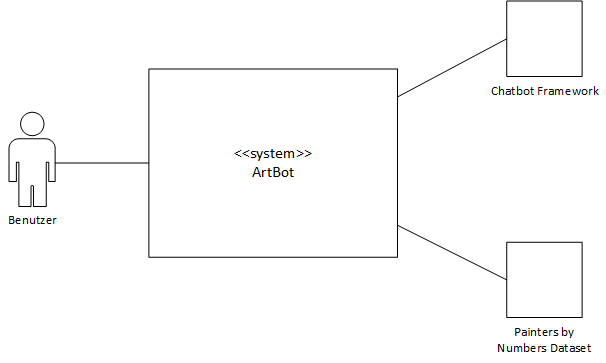
\includegraphics[width=0.6\linewidth]{figures/fachKontext.png}}
	\caption{Fachlicher Kontext von ArtBot}
	\label{fachKontext}
\end{figure}
	
\paragraph{Menschlicher Anwender(Benutzer)}
ArtBot ist ein Chatbot, dessen Funktion es ist, auf Nachfrage Bilder von berühmten Künstlern auszugeben. Dafür muss ein Benutzer mit ArtBot interagieren und über ein Chatfenster die nötigen Informationen eingeben.  

\paragraph{Chatbot Framework - Rasa (Fremdsystem)}
Die Grundlage für den Chatbot bildet ein Framework, hier haben wir uns für Rasa entschieden. Ein Framework vereinfacht die Erstellung des Chatbots, indem es ein Grundgerüst mit den wichtigen Funktionen bereitstellt.

\paragraph{Painter by Numbers (Datensatz)}
Die Grundlage für die Daten des Chatbots bildet ein Datensatz, der auf der Webseite Kaggle.com veröffentlicht wurde. Dieser Datensatz enthält Bilder von berühmten Künstlern zusammen mit diversen Hintergrundinformationen. Dieser Datensatz wird in \ref{daten} genauer beschrieben.
\newpage

\subsection{Technischer Kontext}
\begin{figure}[H]
	\centerline{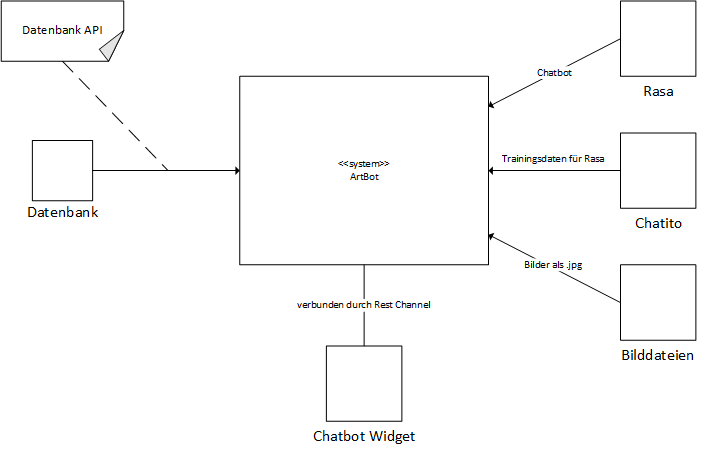
\includegraphics[width=0.9\linewidth]{figures/techKontext.png}}
	\caption{Technischer Kontext von ArtBot}
	\label{techKontext}
\end{figure}

\paragraph{Rasa}
Wie in \ref{fach_text} bereits erwähnt, haben wir uns bei der Wahl unseres Frameworks für Rasa entschieden \cite{rasa_mainpage}. Dabei war wichtig, dass das Framework Open Source ist und es eine solide Grundlage mit guter Erweiterbarkeit bietet. Rasa ist ein Framework für automatisierte Konversationen, welches auf Machine Learning basiert. Der genaue Aufbau von Rasa sowie die Erweiterung werden in späteren Kapiteln detaillierter beschrieben.

\paragraph{Chatito}
Da für Rasa Trainingsdaten und Testdaten benötigt werden und es sehr mühsam ist diese von Hand zu schreiben, haben wir Chatito verwendet, um diese zu generieren. Chatito ist eine Online Anwendung, die unter \cite{chatito_ide} aufrufbar ist. Diese Anwendung erleichtert das Erstellen von Datensätzen ungemein, indem sie aus einigen vom Benutzer eingegebenen Wörtern Datensätze erstellt, welche dann direkt mit Rasa (und auch anderen Frameworks) verwendet werden können. Dieser Vorgang wird in \ref{chatito} genauer beschrieben.

\paragraph{Datenbank}
Die grundlegenden Daten und Bilder die für ArtBot zum Einsatz kommen, entstammen einem Datensatz, welcher in \ref{daten} genauer beschrieben wird. Die Daten dieses Datensatzes haben wir gekürzt und die relevanten Informationen in eine Datenbank geschrieben. Das Modell dieser Datenbank wird in \ref{datenbankmodell} genauer erläutert.

\paragraph{Bilddateien}
Die zu den Daten in der Datenbank zugehörigen Bilder, welche auch aus dem Kaggle Datensatz stammen, sind in einem extra Ordner abgelegt. Diese werden über den Dateinamen, welcher auch in der Datenbank hinterlegt ist, zugeordnet. 

\paragraph{Chatbot Widget}
Da der grundlegende Chatbot, welcher mit Rasa entwickelt wurde, nur auf der Kommandozeile arbeitet, wird ein Frontend benötigt, um Bilder auszugeben. Für diesen Zweck haben wir das Chatbot Widget verwendet. Das ist ein Frontend für Rasa, welches im Browser ausgeführt wird, auf Javascript, HTML sowie CSS basiert und mithilfe von Rest Channels mit Rasa kommuniziert. Dies wird in \ref{chatbot_widget} genauer beschrieben. Dieses Frontend stammt von Jitesh Gaikwad und wurde auf Github unter \cite{chatbot_widget} veröffentlicht.

\subsection{Datengrundlage}\label{daten}
Wie bereits vorher erwähnt, basieren die Daten, welche dem ArtBot zur Verfügung stehen, auf einem Datensatz der auf der Website Kaggle.com veröffentlicht wurde. Der Name des Datensatzes ist Painter by Numbers und er wurde im Rahmen eines Wettbewerbs erstellt. Bei diesem Wettbewerb sollte ein Algorithmus entwickelt werden, der Bilder paarweise überprüft, ob diese vom gleichen Künstler sind. Dafür wurde ein großer Datensatz mit über 2000 Künstlern und über 10000 Bildern sowie zahlreiche Zusatzinformationen bereitgestellt. Dabei war der Datensatz bereits in Trainings- und Testdaten für den Fall des Wettbewerbs aufgeteilt. Der Datensatz ist unter \cite{datensatz} zu finden und die Struktur der Hauptdatei all\_data\_info.csv ist in \ref{datensatz} abgebildet. Für das Projekt waren nur die Hauptdatei, sowie die einzelnen Bilder interessant. Für die Zwecke von ArtBot haben wir zuerst die Attribute date, pixelsx, pixelsy, size\_bytes, source, artist\_group und in\_train entfernt. Zusätzlich wurden alle Einträge entfernt, welche leere Felder beinhalten. Daraufhin haben wir 20 Künstler mit jeweils 5 Bildern ausgewählt und diese als unseren Datensatz für ArtBot gewählt.

\begin{figure}[H]
	\centerline{\includegraphics[width=1.0\linewidth]{figures/datensatz.png}}
	\caption{Aufbau der Hauptdatei all\_data\_info.csv}
	\label{datensatz}
\end{figure}